\subsection{Implementation and Deployment}
\label{sec:deployment}

\begin{figure}[t]
  \centering
  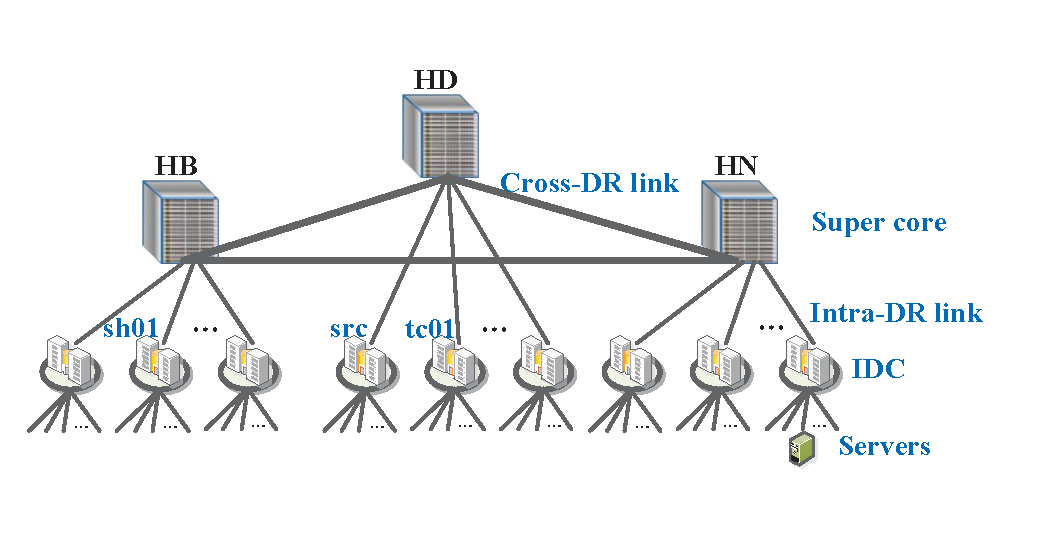
\includegraphics[width=3in]{images/Testbed_v2.eps}
  \caption{The abstract topology of our intra-net WAN.}
  \label{fig:topology}
\end{figure}
%\vspace{-15pt}

We have deployed \name on \company's DCs, which consist of 67 geo-distributed servers in 10. The topology is shown as Fig. \ref{fig:topology}. Evaluations in the next section are based on this deployment.

\name is implemented with 3621 lines of golang code \cite{golang}, and can be fully integrated in \company's DCs. The three duplications of the controller are implemented on three geo-located different servers. The data plane (bulk data transmissions) between controller and agents adopts TCP, and the control plane (control messages) adopts HTTP. For the specific transmissions, \name uses \emph{wget} to make data transfer and sets particular \emph{wget options} to enforce bandwidth.

This implementation makes no specific requirements on applications, and each application that needs to distribute bulk data distribution just follows three steps: 1. register on \name, initiate the basic information about source DC, all end servers and the bulk data. 2. install agents on the involved end servers, 3. assign the start time of bulk data transmission. Then \name will start the data distribution at the specified time. Such simple implementation also makes \name applicable to other companies' DCs. 	

%\jc{this is oversimplistic. did you make any assumption about the agent? what if a hadoop application wants to use your stuff?}

%\jc{a missing piece is what's application interface. if an application wants to send a file, does it make a function call to your system?}

%\jc{what changes did you make on each server? where was the controller implemented? what's the protocol? how did data transfer happen (wget?)? how was bandwidth enforcement done (wget option)? }



%
%\begin{itemize}
%\item \name consists of \fillme line of \fillme code, and can be fully integrated in \company's DCs.
%
%\item Application interfaces: What information does an application need to announce to \name to initiate a multicast.
%
%\item What's the software platform to implement each component
%
%\item Why \name is also applicable to other DCs?
%
%\end{itemize}

